\subsection{\textit{Mari0}: \textit{Mario Bros} con portales}

Tal y como hemos explicado anteriormente, este videojuego es la combinación entre los videojuegos \textit{Mario Bros} y \textit{P0rtal}. Al ser una combinación entre estos videojuegos comparte muchos de sus elementos, entre ellos sus objetivos. El objetivo de estos videojuegos es llegar al final de cada nivel. En cada nivel se proponen diferentes retos y usando los elementos del entorno disponibles y las mecánicas propias del juego, se deben resolver estos retos. El juego está limitado a 4 jugadores como máximo.

\subsubsection{Mecánicas}

Las mecánicas principales de este juego son el movimiento básico del Mario y la pistola de portales. El movimiento básico consiste en el movimiento a izquierda o derecha y el salto. La pistola de portales es algo más compleja. 

\subsubsection*{Movimiento y acciones}

El movimiento y las acciones básicas de este juego son más variadas que en juegos similares. Algunas de estas acciones no se han implementado en el entorno porque añadían demasiada complejidad al entorno o simplemente porque no aportaban ninguna ventaja. Las principales acciones que se pueden realizar son:

\begin{itemize}
    \item \textbf{Movimiento}: Moverse a la derecha o izquierda.
    \item \textbf{Sprint}: cuando se está moviendo hacia alguna dirección es posible esprintar. Esta acción no está implementada en el entorno.
    \item \textbf{Salto alto}: Este es el salto en el cual se llega a máxima altura. Este es el único tipo de salto que está implementado en el entorno.
    \item \textbf{Salto bajo}: Si una vez presionado el botón de salto, se deja de presionar, el jugador realiza un salto de menor altura. Este tipo de salto no está implementado.
    \item \textbf{Usar objeto}: Esta acción usa el objeto que está más cerca del jugador. Se usa principalmente para agarrar cajas y accionar pulsadores.
    \item \textbf{Ataque}: Esta acción solo puede usarse cuando el jugador está en el estado de Mario de fuego. El jugador suelta una bolita de fuego que rebota y daña a los enemigos que golpee. Esta acción no está implementada en el entorno.
    \item \textbf{Portal 1 y 2}: Con esta acción el jugador dispara su portal 1 o 2 en un ángulo desde su posición.
    \item \textbf{Recargar portales}: Con esta acción el jugador retira todos los portales que haya colocado.
\end{itemize}

\subsubsection*{Portales}

Cada jugador dispone de una pistola con dos tipos de portales, el portal izquierdo y el derecho o portales 1 y 2, cada uno representado con un color distinto. Estos portales se pueden atravesar por los todos los jugadores y por otros elementos como cajas y láseres. En la Figura \ref {fig:portal} podemos ver mejor el funcionamiento de un portal.
\begin{figure}[h]
    \centering
    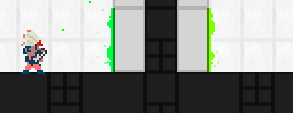
\includegraphics[width=0.9\textwidth]{img/portal-function.png}
    \caption{Funcionamiento de un portal [Elaboración Propia]}
    \label{fig:portal}
\end{figure}

Si el jugador que aparece en la Figura \ref{fig:portal} atraviesa uno de los lados del portal, aparecerá en el otro lado del portal manteniendo la dirección del movimiento y su velocidad. Extrapolando este conocimiento, cuando un jugador atraviesa un portal, la magnitud de su velocidad se mantendrá intacta al salir por el otro lado del portal, mientras que su dirección estará dictada por la dirección en la que está enfocada el portal de salida.

Aunque los portales son una gran herramienta, también tienen sus limitaciones. Las principales limitaciones que hemos encontrado son:

\begin{itemize}
    \item Los portales solo pueden colocarse sobre superficies de color grisáceo como la que podemos ver en la Figura \ref{fig:portal}.
    \item No es posible disparar proyectiles de portales a través de un portal abierto.
    \item Cada jugador solo puede tener colocado únicamente 1 portal de cada tipo a la vez. Además, los proyectiles de los portales viajan únicamente en línea recta.
    \item Existen algunos elementos que no permiten que los proyectiles de portales los atraviesen y cuando un jugador pasa a través de estos, todos los portales colocados por este jugador se eliminan. Adicionalmente, el jugador dispone de una tecla para eliminar todos los portales colocados voluntariamente.
\end{itemize}


\subsubsection{Elementos del entorno}

\subsubsection*{Láseres azules}

Estos láseres son tangibles por los jugadores y por lo tanto pueden servir como plataforma o como obstáculo. Adicionalmente, estos láseres pueden atravesar portales dándoles mucha más utilidad. Finalmente, los proyectiles de portales pueden atravesar estos láseres sin sufrir ninguna consecuencia. En la figura \ref {fig:laser-azul} podemos ver un ejemplo de estos láseres.
\begin{figure}[h]
    \centering
    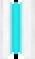
\includegraphics[width=0.1\textwidth]{img/laser-azul.png}
    \caption{Láser azul de \textit{Mari0} [Elaboración Propia]}
    \label{fig:laser-azul}
\end{figure}

\subsubsection*{Láseres anti-portales}

Estos láseres son elementos que los jugadores pueden atravesar pero con ciertas consecuencias. En primer lugar, los proyectiles de portales no pueden atravesar estos láseres. Adicionalmente, cuando un jugador los atraviesa, eliminan todos los portales colocados por este jugador. Este láser es muy útil en la creación de niveles y sobre todo para prevenir situaciones extrañas donde un jugador sea teletrasportado a una parte del nivel que ya se haya superado.
\begin{figure}[h]
    \centering
    
\includegraphics[width=0.1\textwidth]{img/laser-antiportal.png}
    \caption{Láser anti-portal de \textit{Mari0} [Elaboración Propia]}
    \label{fig:antiportal}
\end{figure}

\subsubsection*{Elementos accionadores}

Dentro del entorno existen varios elementos que se pueden accionar, desencadenando así una reacción. Los elementos más comunes son botones y pulsadores. Los primeros se accionan cuando tienen un jugador o una caja encima de ellos mientras que los últimos se accionan mediante la tecla de uso del jugador. Ambos disponen a su vez de una línea que sirve para indicar que elemento accionan. Podemos ver ejemplos de estos elementos en la figura \ref {fig:boton}.
\begin{figure}[h]
    \centering
    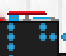
\includegraphics[width=0.1\textwidth]{img/boton.png}
    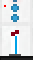
\includegraphics[width=0.05\textwidth]{img/pulsador.png}
    \caption{Botón y pulsador de \textit{Mari0} [Elaboración Propia]}
    \label{fig:boton}
\end{figure}

Además de estos elementos que hemos explicado, existen muchos otros como los geles, cajas, láseres rojos, palancas de salto, láseres anti-gravitatorios etc. El objetivo de este apartado no es explicar todos los elementos que existen sino solo los principales. Con los elementos que hemos explicado hasta ahora es suficiente para continuar nuestra explicación del diseño del entorno. 

